\documentclass[a4paper, 11pt]{article}
\usepackage[margin=0.5in]{geometry}
\usepackage{framed}
\usepackage{graphicx}
\usepackage{subcaption}
\usepackage[brazil]{babel}
\usepackage{xcolor}
\usepackage{blindtext}
\usepackage{xcolor}
\usepackage{mdframed}
\usepackage{indentfirst}
\usepackage{hyperref}
\usepackage{txfonts}
\usepackage{amsmath}
\usepackage{titling}
\usepackage{titlesec}


\definecolor{LightGray}{gray}{0.97}
\usepackage{minted}

\usepackage{xcolor} % to access the named colour LightGray

\setminted[fortran]{  framesep=2mm,
  baselinestretch=1.2,
  bgcolor=LightGray,
  fontsize=\footnotesize,
  linenos}


\graphicspath{ {./graficos/} }
\titleformat{\section}{\normalfont\Large\bfseries}{\thesection}{1em}{}[\titlerule] 
\titleformat{\subsection}{\normalfont\large\bfseries}{\thesubsection}{1em}{} 
% \renewcommand\thesubsection{\Alph{subsection}}
\begin{document}
\noindent
\large\textbf{Autor:} Jefter Santiago \hfill \textbf{PROJETO 1 : {\color{blue} \emph{Análise espectral por transformadas de fourier}}}   \\
\#USP: 12559016 \\
\normalsize Curso: Física Estatística Computacional \\
Prof. F. C. Alcaraz \hfill Data de entrega: 23/03/2024 \\
\noindent\rule{7in}{2.8pt}

\begin{abstract}
  Nesse trabalho foi estudada a transformada de Fourier discreta. Implementamos um algoritmo
  da transformada e sua inversa e foram feitas análises espectrais de sinais gerados a partir
  de uma função simples. Nesse processo conseguimos observar as consequências do teorema de
  amostragem de Nyquist-Shannon ao aplicarmos a transformada de fourier para um conjunto finito
  de pontos. Para finalizar foram feitas análises de desempenho dos algoritmos utilizados
  e demonstrado que crescimento do número de passos a partir do número de pontos é quadrático.
\end{abstract}

\section{Discretização da transformada de Fourier}

Partindo da transformada de Fourier(\ref{eq:transformada_fourier}) realizamos a discretização
da mesma

\begin{equation}
  y(t) = \int_{-\infty}^{\infty}Y(f) e^{-2\pi i f t} df = \frac{1}{2\pi}\int_{-\infty}^{\infty} Y(\omega/2\pi) e^{-i\omega t} d \omega
  \label{eq:transformada_fourier}
\end{equation}



Buscando uma formula discretizada para a transformada de Fourier.

Dividimos os eixo temporal em $N$ tempos diferentes, trabalharemos
com passos de mesmo tamanho \( \Delta t \), onde \( t_\ell = \ell \Delta t \) é o tempo
a cada iteração. Para um numero fixo de passos $N$, em um intervalo
de \( [a, b] \) podemos fixar \( \Delta t = \frac{b}{N} \).
\[
  Y(f) = \frac{b}{N}  \sum_{\ell= 0}^{N - 1} y_\ell e^{2 \pi i(b\ell/N)}
\]

Segue que a frequência discretizada pode ser dada por \( f_k = \frac{k}{N\Delta t} = \frac{k}{b}\), \( k = 0, 1, \cdots , N-1
\). Fazendo \( \tilde{Y_k} = \left( N/b \right) Y_k \), a relação
para a transformada fica

\[ Y_k \left( \frac{N}{b} \right) = \tilde{Y_k} = \sum_{\ell = 0}^{N-1} y_\ell e^{2\pi i \left( k\ell/N \right) } \]

portanto, denotamos a transformada e a inversa dela simplesmente por 

\begin{equation}
  Y_k = \sum_{\ell = 0}^{N-1} y_\ell e^{2\pi i \left( k\ell/N \right)}
  \label{eq:dft} 
\end{equation}
\begin{equation}
  y_\ell = \frac{1}{N} \sum_{k=0}^{N-1} Y_k e^{-2\pi i \left( kj/N \right)}
  \label{eq:idft} 
\end{equation}

Se estivermos trabalhando com sinais puramente reais todas componentes imaginárias serão
nulas. Já se o sinal for complexo, podemos realizar a transformada(\ref{eq:dft}) em apenas
metade dos pontos e obter as componentes corretas, adicionando distorções no espectro do sinal e
consequentemente na transformada inversa. No entando, se realizarmos a transformada apenas com metade
desses pontos não seria possível reconstruir a função usando a (\ref{eq:idft}), pois não seria
possível representar o domínio completo com metade dos pontos.


Por isso não implementei a transformada dessa forma e nos resultados observaram-se os reflexos das
componentes mais de uma vez no domínio, demonstrando a redundância de se realizar a transformação
para pontos com $n \geq N/2$.


Uma definição importante para se estudar o espectro dos sinais é a frequência de Nyquist. Supondo
que trabalhamos com sinais obtidos em tempos \( \Delta t \), como vimos, basta $N/2 - 1$ pontos para
descrever bem as componentes do sinal. O teorema da amostragem de Nyquist-Shannon nos diz qual a
frequência máxima que uma componente de Fourier pode ter.
\[ f =  \left( \frac{N}{2} - 1 \right) \left( N \Delta t\right) \approx \frac{1}{2\Delta t}\]

\begin{equation}
  f_{\text{Nyquist}} \equiv \frac{1}{2 \Delta t}
  \label{eq:fnyquist}
\end{equation}


Foram estudadas as condições em que a frequência de Nyquist (\ref{eq:fnyquist}) não são
satisfeitas e o qual a implicação disso no resultado obtido. Nessa situações não conseguiremos
obter uma representação perfeita das componentes de Fourier do nosso sinal, como esperado.
E pode dificultar a identificação da frequência correta do componente. Esse tipo de problema pode
gerar a representação incorreta da função real que buscaremos aproximar depois.

Quando trabalhamos trabalhamos com sinais com frequência acima da frequência de Nyquist obtemos um
fenômeno de falseamento ou aliasing, dado pelo fato de que mais deu uma função pode passar pelo
ponto amostrado. Nesses casos em que temos uma amostragem pequena podemos usar a frequência
(\ref{eq:fnyquist}) para estimar qual a frequência correta do ponto. Sabendo qual original do sinal
podemos descobrir onde a frequência real será refletida a partir da frequência de Nyquist pela relação

\begin{equation}
f_{\text{real}} = 2 f_{\text{Nyquist}} - f_{\text{Original}}  
\label{eq:achar_frequencia}
\end{equation}

onde a frequência original é dada por um paramêtro conhecido.


Em um cenário real de uso da tranformada poderiámos definir qual a frequência de Nysquit desejamos
trabalhar simplesmente ajustando a amostragem das medições ou simulação. Vimos na discretização que
na série temporal em um intervalo finito definimos o \( \Delta t \) como a ``janela'' ou distância entre
um ponto do sinal e outro. Na prática isso funciona como uma resolução dos experimento, ou seja,
podemos aumentar ou diminuir essa relação de Nysquist conforme necessário.

\section{Gerando séries}

O trabalho foi iniciado gerando todos os sinais com os quais trabalhamos. Em todo o
projeto foram utilizadas séries da forma (\ref{eq:sinais}) usadas para gerar sinais
em que testamos a transformada de Fourier e sua inversa.

\begin{equation}
  y_i = a_1 \cos (\omega_1 t_i)   + a_2 \sin (\omega_2 t_i) , t_i = i \cdot  \Delta t , i = 1, \cdots , N
  \label{eq:sinais}
\end{equation}


Segue na tabela(\ref{tbl:parametros_sinais}) abaixo os paramêtros utilizados para construção dos sinais

\begin{table}[h!]
  \centering
\begin{tabular}{|c|c|c|c|c|c|}
\hline
Parâmetro                       & $\Delta t$                & $a_1$                  & $a_2$ & $\omega_1 (Hz)$ & $\omega_2 (Hz)$ \\ \hline
I                       & 0.04                 & 2                      & 4     & $4\pi$     & $2.5\pi$   \\ \hline
II                       & 0.04                 & 3                      & 2     & $4\pi$     & $2.5\pi$   \\ \hline
III                       & 0.4                  & 2                      & 4     & $4\pi$     & $0.2\pi$   \\ \hline
IV                       & 0.4  & 3 & 2         & $4\pi$                   & $0.2\pi$   \\ \hline
V                       & 0.04 & 2 & 4         & $4\pi$                   & $1.4\pi$   \\ \hline
VI                       & 0.04 & 2 & 4         & $4.2\pi$                 & $1.4\pi$   \\ \hline
\end{tabular}
\caption{Parâmetros dos sinais gerados com $N = 200$ iterações.}
\label{tbl:parametros_sinais}
\end{table}

Código utilizado para gerar {\bfseries todos } sinais a partir da (\ref{eq:sinais}) estudados nesse trabalho.
Esse código está no localizado no diretório \emph{tarefa-2} e gera os arquivos ``.dat'' que podemos
utilizar nos outros programas.

\begin{minted}{fortran}[!]
      parameter(pi = acos(-1e0))
      dimension Ns(1:4)
      parameter(Ns = (/50, 100, 200, 400/))

      open(10, file="output-signal-A.dat")
      open(20, file="output-signal-B.dat")
      open(30, file="output-signal-C.dat")
      open(40, file="output-signal-D.dat")
      open(50, file="output-signal-E.dat")
      open(60, file="output-signal-F.dat")

      dt1 = 0.04
      dt2 = 0.4
      a11 = 2.0e0
      a12 = 3.0e0
      a21 = 4.0e0
      a22 = 2.0e0
      w1 = 4.0e0 * pi
      w21 = 2.5e0 * pi
      w22 = 0.2e0 * pi
      do i = 1, 200
         ti1 = i * dt1
         ti2 = i * dt2
         write(10, *)  ti1, a11*cos(w1*ti1) + a21*sin(w21*ti1) 
         write(20, *)  ti1, a12*cos(w1*ti1) + a22*sin(w21*ti1) 
         write(30, *)  ti2, a11*cos(w1*ti2) + a21*sin(w22*ti2) 
         write(40, *)  ti2, a12*cos(w1*ti2) + a22*sin(w22*ti2) 
         write(50, *)  ti1, a11*cos(w1*ti1) + a21*sin(1.4e0*pi*ti1) 
         write(60, *)  ti1, a11*cos(4.2*pi*ti1) + a21*sin(1.4e0*pi*ti1) 
      end do
      close(10)
      close(20)
      close(30)
      close(40)
      close(50)
      close(60)

      ! Gera os sinais para avaliação do tempo de execução da transformada de Fourier
      ! gera sinal para Ns = 50, ...
      open(1, file="output-signal-n50.dat")
      open(2, file="output-signal-n100.dat")
      open(3, file="output-signal-n200.dat")
      open(4, file="output-signal-n400.dat")
      do k = 1, 4
         do i = 1, Ns(k)
            ti1 = i * dt1
            write(k, *)  ti1, a11*cos(w1*ti1) + a21*sin(w21*ti1) 
         end do
         close(k)
      end do
      end
\end{minted}

Para estudar a implementação do algoritmo da transformada discreta {\bfseries (DFT) } foram gerados
os sinais abaixo.

\begin{figure}[h!]
    \centering
    \begin{subfigure}{0.45\textwidth}
        \centering
        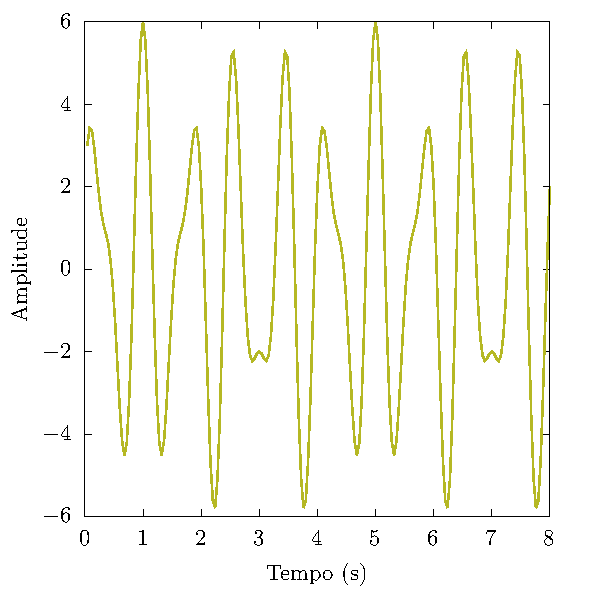
\includegraphics[width=\textwidth]{signal-A}
        \caption{\(a_1=2, a_2 = 4,  \omega_1 = 4\pi (Hz), \omega_2=2.5\pi(Hz)\)}
        \label{fig:subA}
    \end{subfigure}
    \begin{subfigure}{0.45\textwidth}
        \centering
        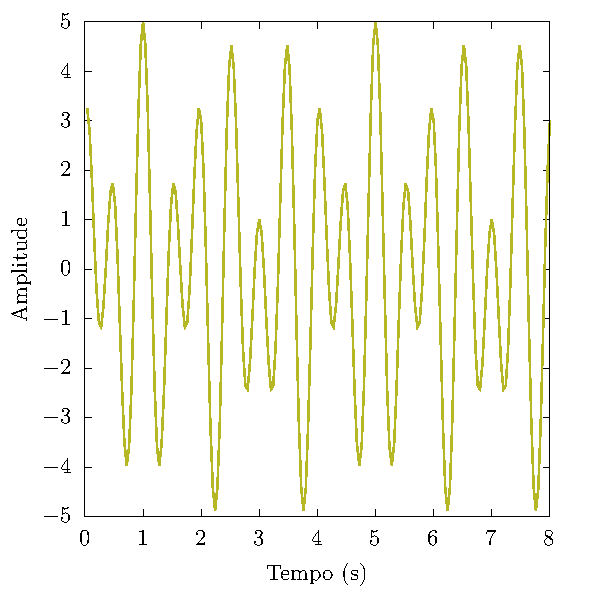
\includegraphics[width=\textwidth]{signal-B}
        \caption{\(a_1 = 3, a_2 = 2, \omega_1 = 4\pi (Hz), \omega_2 = 2.5\pi (Hz)\)}
        \label{fig:subB}
    \end{subfigure}
    \caption{Séries temporais relativas aos parâmetros (I) e (II).}
    \label{fig:sinais_1}
\end{figure}

Nota-se que os sinais utilizados são bem semelhantes, os sinais (\ref{fig:subA}) e (\ref{fig:subB})
tem amplitudes diferentes para os senos e cossenos e as mesmas frequências. 


\begin{figure}[h!]
  \centering
    \begin{subfigure}{0.45\textwidth}
        \centering
        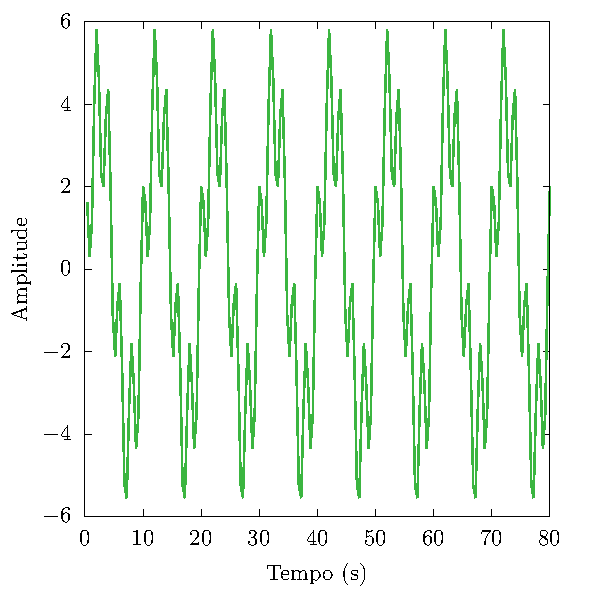
\includegraphics[width=\textwidth]{signal-C}
        \caption{\(a_1 = 2, a_2 = 4, \omega_1 = 4\pi(Hz), \omega_2 = 0.2\pi (Hz)\)}
        \label{fig:subC}
    \end{subfigure} 
    \begin{subfigure}{0.45\textwidth}
        \centering
        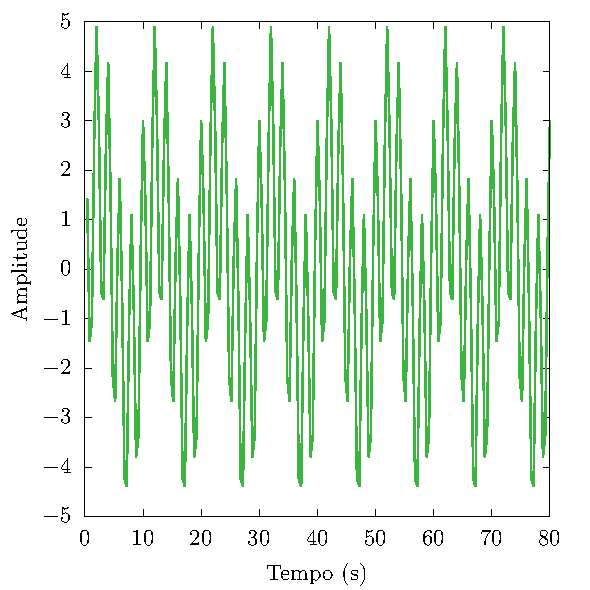
\includegraphics[width=\textwidth]{signal-D}
        \caption{\(a_1 = 3, a_2 = 2, \omega_1 = 4\pi(Hz), \omega_2 = 0.2\pi (Hz)\)}
        \label{fig:subD}
    \end{subfigure}
    \caption{Séries temporais relativas aos parâmetros (III) e (IV).}
    \label{fig:sinais_2}
\end{figure}

Já os sinais (\ref{fig:subC}) e (\ref{fig:subD}) tem frequências menores que os anteriores, mas
mesmas amplitudes que (\ref{fig:subA}) e (\ref{fig:subB}), respectivamente.

\begin{figure}[h!]
  \centering
    \begin{subfigure}{0.45\textwidth}
        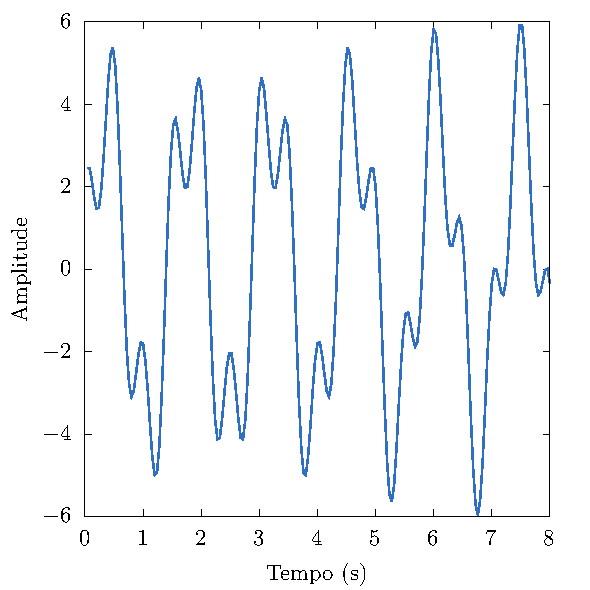
\includegraphics[width=\textwidth]{signal-E}
        \caption{\(a_1 = 2, a_2 = 4, \omega_1 = 4\pi(Hz), \omega_2 = 1.4\pi (Hz)\)}
        \label{fig:subE}
    \end{subfigure}
    \begin{subfigure}{0.45\textwidth}
        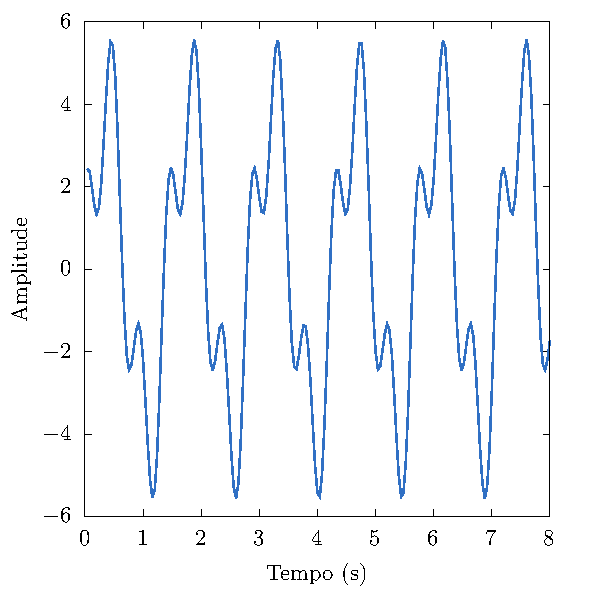
\includegraphics[width=\textwidth]{signal-F}
        \caption{\(a_1 = 2, a_2 = 4, \omega_1 = 4.2\pi(Hz), \omega_2 = 1;4\pi (Hz)\)}
        \label{fig:subF}
    \end{subfigure}
    \caption{Séries temporais relativas aos parâmetros (V) e (VI).}
    \label{fig:sinais_3}
\end{figure}

\section{Implementação da DFT}

Partindo da discretização (\ref{eq:dft}) da transformada de fourier contínua, foi implementada a rotina que
constroí a transformada de Fourier discreta a partir de um conjunto de dados reais com um número
fixo de \( N = 200 \) pontos. Os gráficos das componentes de Fourier para os casos estudados foram
normalizados no eixo $y$ por $100$ buscando facilitar leitura.

O programa foi organizado no diretório \emph{tarefa-1/tarefa1.f} e para executar é necessário que
haja um arquivo de dados nomeado ``data.in'' no mesmo diretório. Os arquivos utilizados para input
de dados são os gerados anteriormente.\footnote{No diretório central do projeto deixei um arquivo
  denotado por \emph{dft.f} e seu executável \emph{dft.exe} que gera as transformadas e sua inversa
  para todos os arquivos de dados que trabalhamos nesse projeto.}

Segue abaixo o código que calcula a \emph{DFT}:
\begin{minted}{fortran}
    implicit real*8(a-h, o-y)
    implicit complex*16(z-z)
    parameter(N = 200)
    parameter(pi = acos(-1.0e0))
    dimension signal(N)
    dimension zYn(N)
    zi = (0.0, 1.0)
    
    open(unit=1, file="data.in")
    open(unit=2, file="data.out")
    
    do i = 1, N
      read(1, *) t, signal(i)
    end do
    dt = t / N
    
    zeta = exp(2*pi*zi/N)
      do l = 1, N
         zYl = signal(1)
         do m = 1, N
            zYl = zYl+signal(m)*zeta**(m*l)
         end do
         zYn(l) = zYl
         write(2, *) l/(N*dt*2*pi),real(zYl),aimag(zYl)
      end do

      close(1)
      close(2)
      end
\end{minted}

O espectro(\ref{fig:espectro1}) é bastante simples e com boa amostragem, as frequências são todas nulas exceto pelas duas
correspondentes às do nosso sinal e nota-se que a única diferença é a amplitude de um seno.

\begin{figure}[h!]
    \centering
    \caption{Componentes de Fourier para os sinais (\ref{fig:subA}) e (\ref{fig:subB}) em um período.}
    \begin{subfigure}{0.45\textwidth}
        \centering
        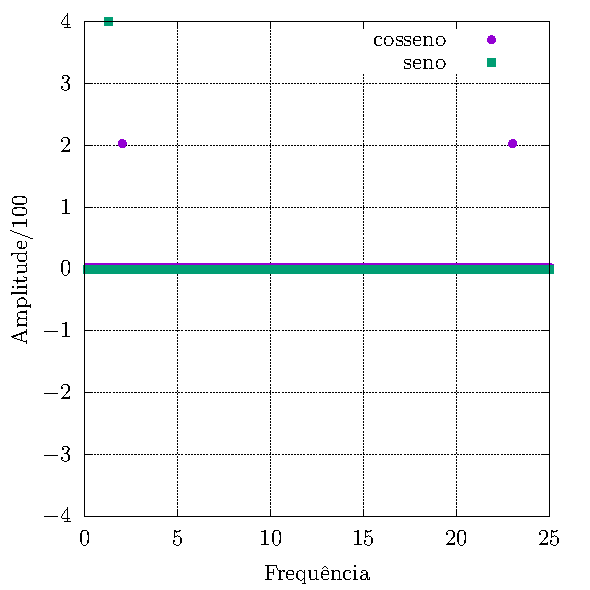
\includegraphics[width=\textwidth]{output-dft-A}
        \caption{Espectro de(\ref{fig:subA}).}
        \label{fig:espectroA}
    \end{subfigure}
    \hfill
    \begin{subfigure}{0.45\textwidth}
        \centering
        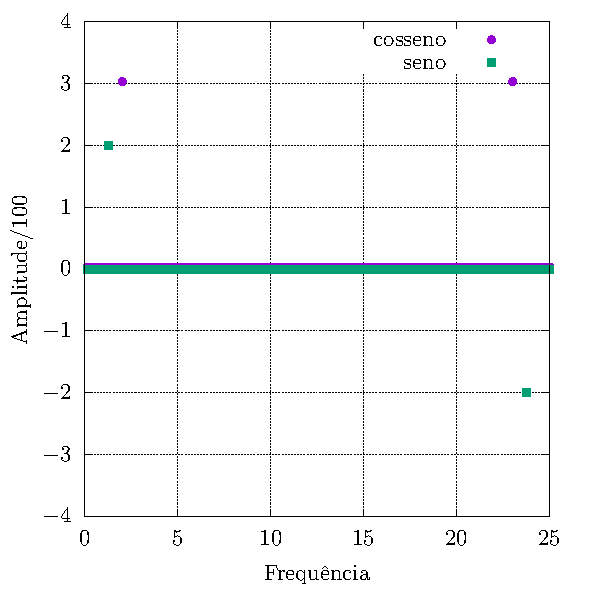
\includegraphics[width=\textwidth]{output-dft-B}
        \caption{Espectro de(\ref{fig:subB}).}
        \label{fig:espectroB}
    \end{subfigure}
        \label{fig:espectro1}
\end{figure} 

Já as componentes de Fourier da figura abaixo (\ref{fig:espectro2}), 
temos que (\ref{eq:fnyquist}) é $f_{\text{Nyquist}} = 1/(2\cdot 0,4) = 1,25 $ e frequência original
é a mesma do sinal estudado anteriormente, pois que a componente do cosseno é a mesma, \(
f_{\text{Original}} =  2 \), portanto o ponto de reflexão é \( f = 2,5 - 2 = 0,5 \). 

\begin{figure}[h!]
    \centering
    \caption{Componentes de Fourier para os sinais (\ref{fig:subC}) e (\ref{fig:subD}).}
    \begin{subfigure}{0.45\textwidth}
        \centering
        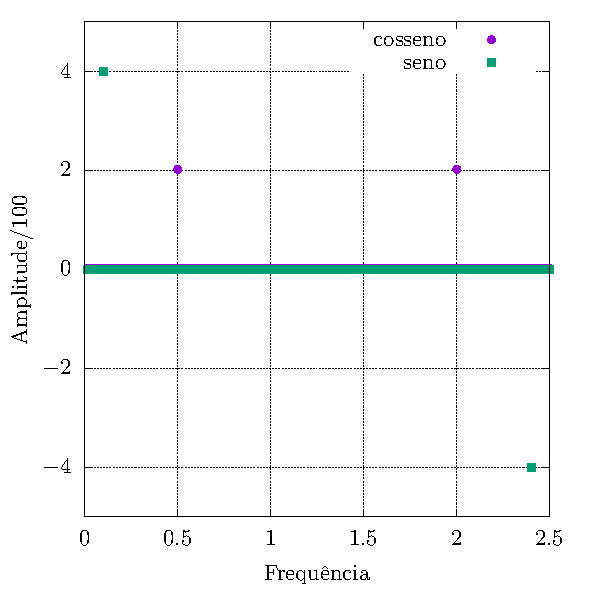
\includegraphics[width=\textwidth]{output-dft-C}
        \caption{Espectro de(\ref{fig:subC}).}
        \label{fig:espectroC}
    \end{subfigure}
    \hfill
    \begin{subfigure}{0.45\textwidth}
        \centering
        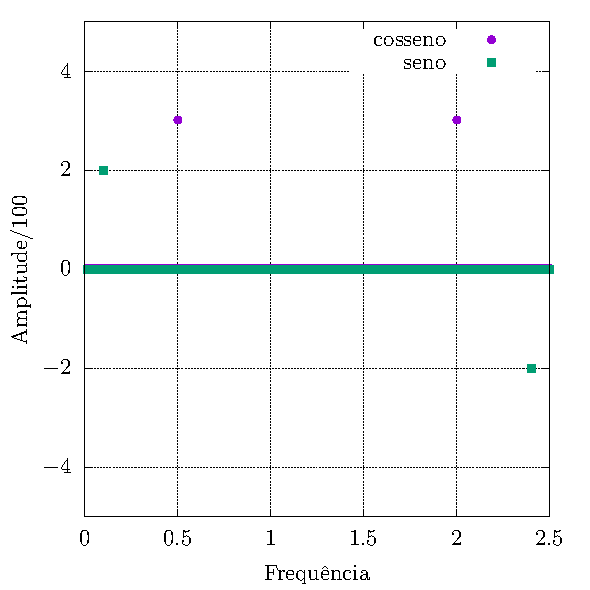
\includegraphics[width=\textwidth]{output-dft-D}
        \caption{Espectro de(\ref{fig:subD}).}
        \label{fig:espectroD}
    \end{subfigure}
   \label{fig:espectro2}
\end{figure} 


Por último, temos os seguintes espectros (\ref{fig:espectro3}). O sinal que gera esses espectros
são bastante parecidos exceto por uma das frequências do (\ref{fig:espectroF}). A partir do
espectro (\ref{fig:espectroE}) a componente do cosseno apresenta mesma frequência que as do sinal
trabalhado anteriormente (\ref{fig:espectroA}) e então sabemos que frequência \( f = 2 \) já pode
ser identificada como um dos picos do cosseno. Outro pico para o seno em \( f = 0,7 \).


Outros pontos não nulos próximos dos picos existem porque a exponencial complexa pode ser interpretada como
somas de cossenos e senos pela relação de Euler, que na prática, faz com que a somatória se torne
somas dessas funções com fases \( \phi \) adicionadas, isso faz com que o sinal não seja nulo e o
espectro se torne menos simples do que para senos e cossenos puros. 

Para o caso do espectro (\ref{fig:espectroF}) temos as componentes com frequências que são o dobro
da outras, isso faz com que ja um comportamento parecido das funções com uma fase somada, que pode
ser visto no zoom da figura. Obtemos as frequência \( f = 2,1\) e \( f = 0.7 \) assim como nos casos
estudados antes. Essa harmônia entre as componentes da transformada dificultam a análise espectral,
já que não temos uma frequência fixa que descreve totalmente o sinal, como em
(\ref{fig:espectroA}).

\begin{figure}[h!]
  \centering
  \caption{Espectros gerados pela {\bfseries DFT } de alguns sinais da figura (\ref{fig:sinais_3})
    em dois períodos completos.}
  \begin{subfigure}{0.45\textwidth}
    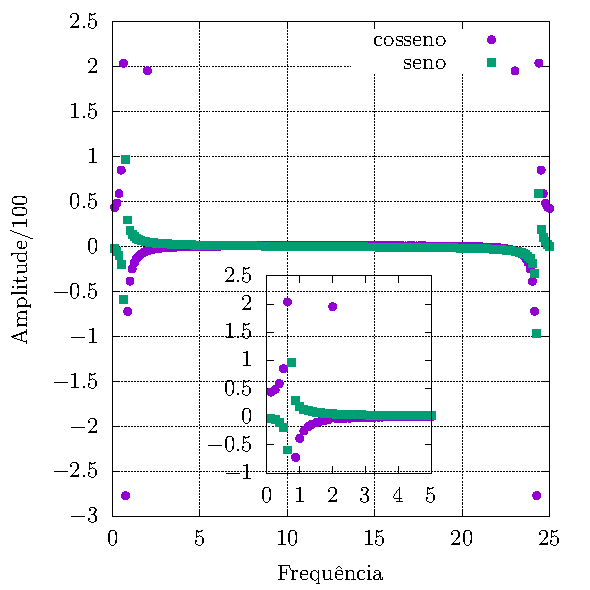
\includegraphics[width=\textwidth]{output-dft-E}
    \caption{Espectro de(\ref{fig:subE}).}
    \label{fig:espectroE}
  \end{subfigure}
  \hfill
  \begin{subfigure}{0.45\textwidth}
    \centering
    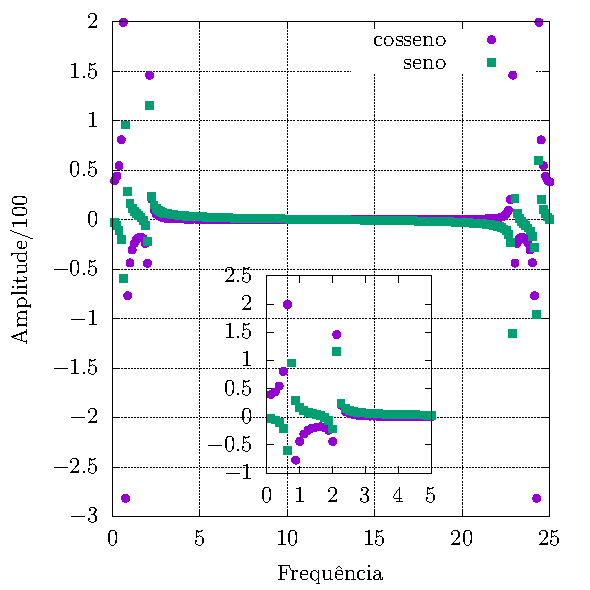
\includegraphics[width=\textwidth]{output-dft-F}
    \caption{Espectro de(\ref{fig:subF}). }
    \label{fig:espectroF}
  \end{subfigure}
  \label{fig:espectro3}
\end{figure}

Nas figuras desses últimos espectros optei por plotar a transformada(\ref{fig:espectro3}) do sinal
com dois periodos completos para apontar algo que aconteceu com todos os sinais: a troca de sinal.
Parte dos sinais são refletidos, invertidos, isso se dá pelas componentes envolvendo o seno que
pela paridade da função muda o sinal. Isso pode ser exemplificado
partindo da (\ref{eq:dft}) e supondo uma componente $N-k$:
\begin{align*}
  Y_{N-k} &= \sum_{\ell = 0}^{N-1} \cos \left( \omega_1 t_\ell \right) \sin \left( 2 \pi \left( \frac{N-k}{N}
            \right) \ell \right) 
          = \sum_{\ell = 0}^{N-1} \cos(\omega_1 t_\ell) \sin \left( 2 \pi \ell  - 2 \pi \frac{k}{N} \ell \right) \\
          &= - \sum_{\ell=0}^{N-1} \cos (\omega_1 t_\ell) \sin \left( \frac{2\pi k}{N}\ell  \right) =  - Y_N
\end{align*}


Apeasar da nuances que surgem na análise das componentes espectrais da transformada de Fourier nos
casos trabalhados, a transformada inversa pode ser obtida perfeitamente por todos os espectros que
obtivemos.


\clearpage
\section{Transformada inversa}


Nessa etapa foi realizada a transformada inversa dos sinais obtidos. O código abaixo
realiza essa rotina e está organizado no diretório \emph{tarefa-4/tarefa4.f}. Ele usa o arquivo
gerado pela rotina da transformada em \emph{tarefa-1/tarefa1.f}, ou seja, o arquivo no local
\emph{tarefa-1/data.out} e gera outro arquivo com o mesmo nome, mas no diretório \emph{tarefa-4}. 


Calcula a inversa da transformada de Fourier a partir dos dados da transformada em um
arquivo ``data.out''. Escreve a transformada inversa e escreve no arquivo ``data.out''.
\begin{minted}{fortran}
      implicit real*8(a-h, o-y)
      implicit complex*16(z-z)
      parameter(N = 200)
      parameter(pi = acos(-1.0e0))
      dimension signal(N)
      dimension zYn(N)
      zi = (0.0, 1.0)

      open(10, file="data.out")

      comp_real = 0.0d0
      comp_imag = 0.0d0

      t = 0.0e0
      do i = 1, N
         read(10, *) t, comp_real, comp_imag
         zYn(i) = cmplx(comp_real, comp_imag)
      end do
      dt = t / N

      zeta = exp(-2*pi*zi/N)
      ! Calcula a transformada inversa
      do m = 1, N
         zYm = zYn(1)/N
         do l = 1, N
            zYm = zYm+zYn(l)*zeta**(m*l)
         end do
         zYm = zYm/N
!     Escreve a transformada inversa no arquivo "data.out"
         write(10, *) m * dt, real(zYm)
      end do
      close(10)
      end
\end{minted}


Executando o programa a partir do espectro do sinal (\ref{fig:subA}) obtemos o resultado abaixo, na
figura (\ref{fig:idft}). É notável que o sinal original é perfeitamente reconstruido a partir da
transformada. E esse é de fato o caso.


\begin{figure}[h!]
  \centering
  \caption{}
  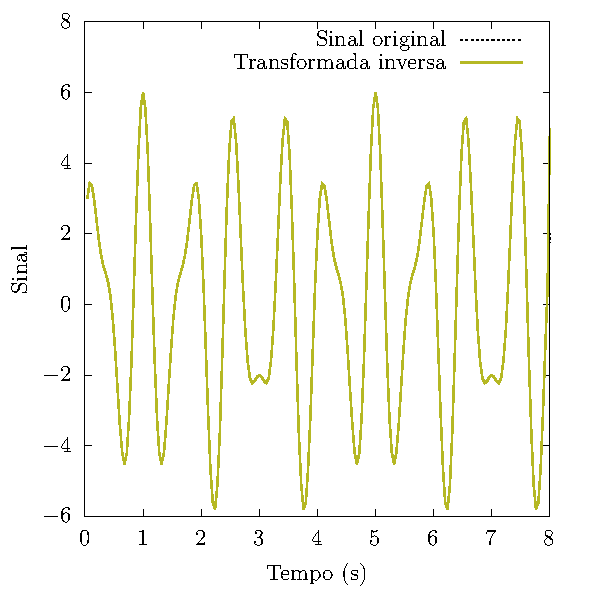
\includegraphics[width=0.30\textwidth]{inv-dft-A}
  \label{fig:idft} 
\end{figure}

Por ilustração também foram feitas gráficos para as transformadas inversas dos outros sinais
gerados:

\begin{figure}[h!]
    \centering
    \begin{subfigure}{0.40\textwidth}
        \centering
        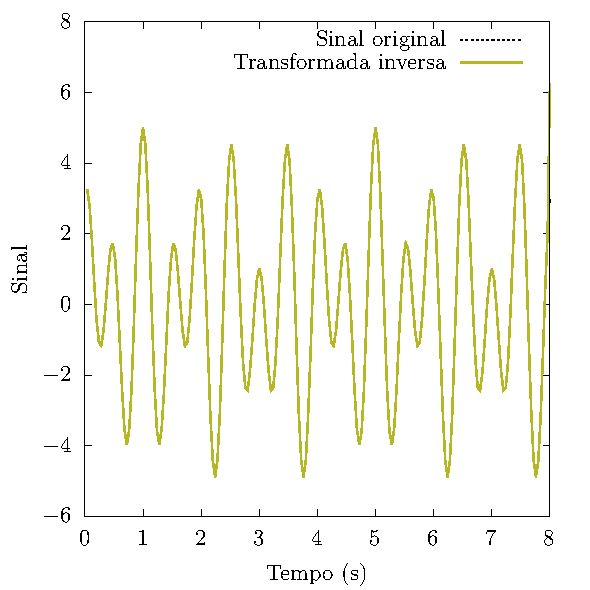
\includegraphics[width=\textwidth]{inv-dft-B}
    \end{subfigure}
    \hfill
    \begin{subfigure}{0.40\textwidth}
        \centering
        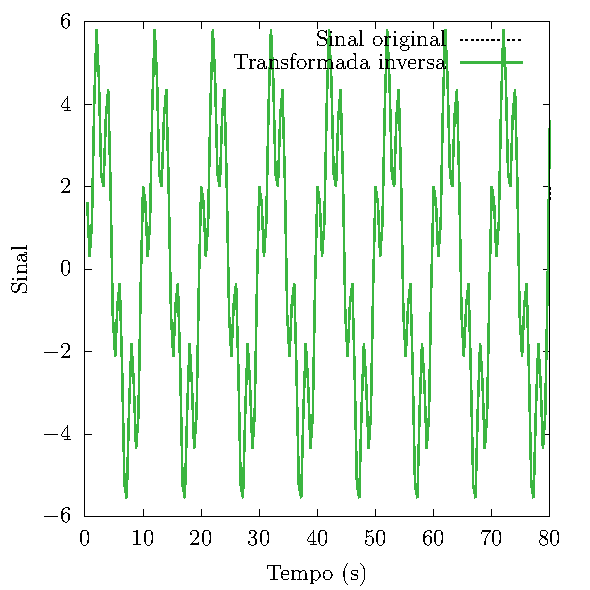
\includegraphics[width=\textwidth]{inv-dft-C}
    \end{subfigure}
    \begin{subfigure}{0.40\textwidth}
        \centering
        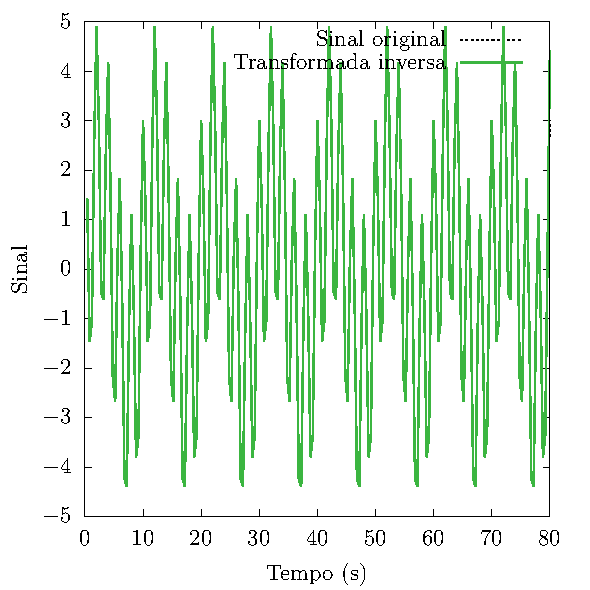
\includegraphics[width=\textwidth]{inv-dft-D}
    \end{subfigure}
    \begin{subfigure}{0.40\textwidth}
        \centering
        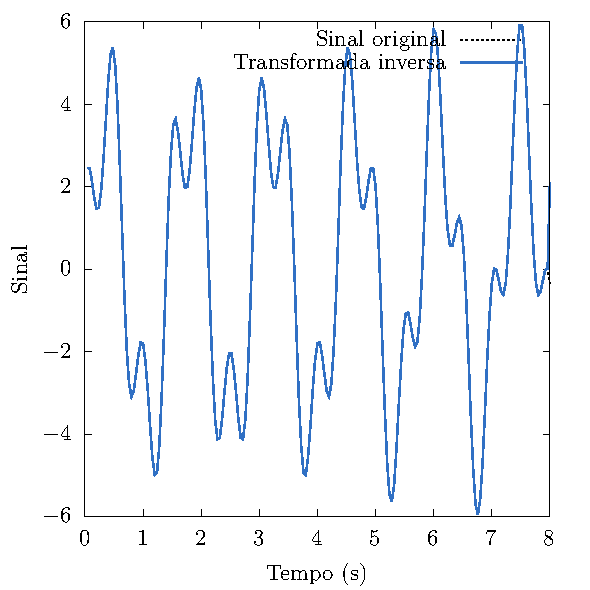
\includegraphics[width=\textwidth]{inv-dft-E}
    \end{subfigure}
    \begin{subfigure}{0.40\textwidth}
        \centering
        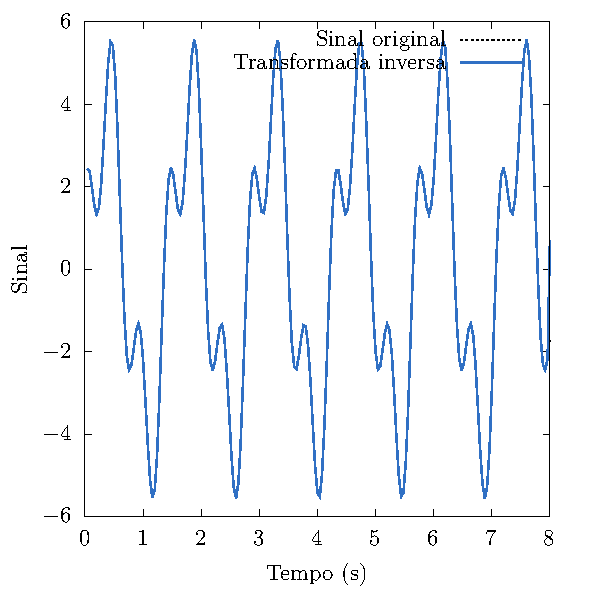
\includegraphics[width=\textwidth]{inv-dft-F}
    \end{subfigure}
    \caption{Transformadas inversas dos sinais de paramêtros (I) à (VI).}
\end{figure}


Não estudamos como avaliar o quão boa é a convergência, mas apenas observados os gráficos é
perceptível que o sinal é perfeitamente reproduzido.

\clearpage
\section{Cálculo do tempo de execução}

Por fim, foi estudado o tempo de execução do algoritmo da tranformada de Fourier. O objetivo do
projeto não era buscar formas eficientes de implementar o algoritmo e por isso a única implementação
feita foi a força bruta. Como esperado, pela discretização (\ref{eq:dft}), a complexidade do
algoritmo é \( \mathcal{O}(n^2) \), o tempo deve crescer com o quadrado da entrada.

Para esse objetivo, a rotina abaixo foi escrita, a partir do código realizado para
\emph{tarefa-1}. Com algumas pequenas alterações. Com ele foram gerados sinais de acordo
com os paramêtros de (\ref{fig:subA}), mas alterando o número de iterações $N$.
Note que não é necessário utilizar uma estrutura de vetor para armazenar as componentes de Fourier
para esse problema específico. No entanto a a estrutura foi mantida e os dados são lidos dos
arquivos gerados pelo \emph{tarefa-2/tarefa2.f} são escritos nesse vetor. Isso porque poderia haver
influência da leitura do arquivo na contagem de tempo total de cada transformada. Como estamos
trabalhando vetores de no máximo $400$ componentes foi escolhido maior gasto de espaço a fim de
testar o desempenho temporal desse programa.


\begin{minted}{fortran}
!     Testes de tempo para algoritmo da transformada de Fourier.
      implicit real*8(a-h, o-y)
      implicit complex*16(z-z)
      dimension N(1:4)
      parameter(N = (/50, 100, 200, 400/))
      parameter(pi = acos(-1.0e0))
      dimension signal(400)
      zi = (0.0, 1.0)

      start_time = 0.0e0
      end_time = 0.0e0

      open(5, file="output-benchmarking.dat")

      open(1, file="output-signal-n50.dat")
      open(2, file="output-signal-n100.dat")
      open(3, file="output-signal-n200.dat")
      open(4, file="output-signal-n400.dat")

      dt = 0.04e0
      t = 0.00e0

      do k = 1, 4
!     N atual
         Nc = N(k)
         do i = 1, Nc 
            read(k, *) t, signal(i)
         end do
         close(i)
         call cpu_time(start_time)
!     Calcula transformada
         zeta = exp(2*pi*zi/Nc)
         do l = 1, Nc
            zYl = signal(1)
            do m = 1, Nc
               zYl = zYl+signal(m)*zeta**(m*l)
            end do
         end do
!     Tempo passado
         call cpu_time(end_time)
         total = end_time-start_time
         write(5, *) N(k), total, total ** (0.5)
      end do
      close(5)
      end
\end{minted}


Na figura abaixo (\ref{fig:tempo_execucao}) estão os resultados desses testes. Podemos
constatar a dependência quadrática com o número de iterações.



\begin{figure}[h!]
  \centering
  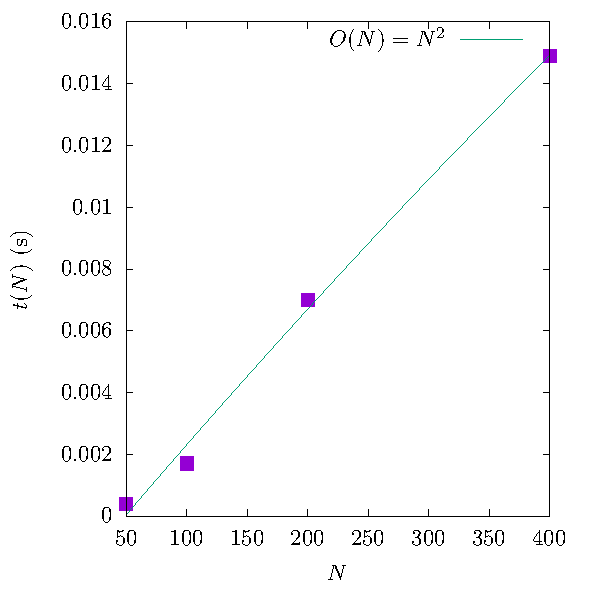
\includegraphics[width=0.55\textwidth]{benchmarking2}
  \caption{Tempo de execução do algoritmo da transformada de Fourier discreta e relação quadrática de crescimento.}
  \label{fig:tempo_execucao}
\end{figure}

Como era esperado a relação entre o número de passos e o tempo é quadrática. Isso já era esperado
pela própria estrutura da discretização (\ref{eq:dft}), que computacionalmente pode ser entendida
como ``nested loops'' ou loops aninhados. Uma possível melhoria para a eficiência de como calculamos
a transformada seria utilizar apenas metade dos pontos, como foi discutido. Porém não teriámos como
construir a função original de volta e no caso asimptótico a relação também seria quadrática.
A solução realmente eficiente seria utilizar do algoritmo {\bfseries FFT}, que manipula as
componentes dos dados tratando as componentes impares e pares de uma forma que é possível realizar
divisão e conquista (ou busca binária) para encontrar as coeficientes de Fourier de um dado
sinal com uma complexidade $\mathcal{O}(N \log_2 N)$. Os detalhes de implementação desse algoritmo está fora
do escopo desse projeto.




\end{document}
%%% Local Variables:
%%% mode: latex
%%% TeX-master: "main.tex"
%%% End:
